\documentclass[tikz,border=10pt]{standalone}
\usepackage{tikz}
\usetikzlibrary{arrows.meta,calc,bending}

\begin{document}

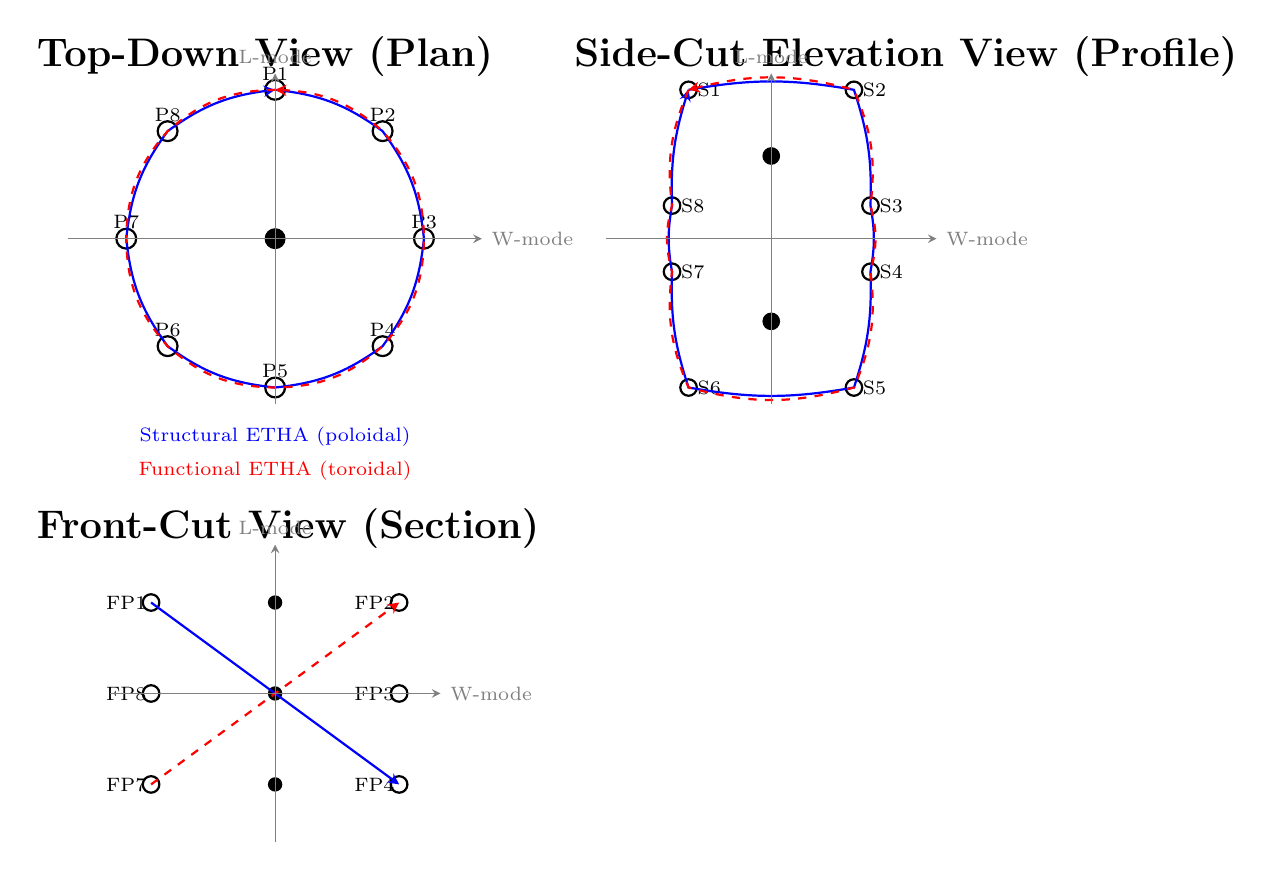
\begin{tikzpicture}[scale=1.05,>=stealth]

% ============================================================
% 1. TOP-DOWN VIEW (PLAN)
% ============================================================

\node[anchor=west] at (-6,5.2) {\Large\textbf{Top-Down View (Plan)}};

% VE chamber
\coordinate (VEtop) at (-3,3);
\filldraw (VEtop) circle (0.12);

% Piston coordinates (explicit, no trig)
\coordinate (P1) at (-3,4.8);
\coordinate (P2) at (-1.7,4.3);
\coordinate (P3) at (-1.2,3);
\coordinate (P4) at (-1.7,1.7);
\coordinate (P5) at (-3,1.2);
\coordinate (P6) at (-4.3,1.7);
\coordinate (P7) at (-4.8,3);
\coordinate (P8) at (-4.3,4.3);

% Draw pistons
\foreach \p in {P1,P2,P3,P4,P5,P6,P7,P8}{
  \filldraw[white] (\p) circle (0.12);
  \draw[thick] (\p) circle (0.12);
  \node[font=\scriptsize,anchor=south] at (\p) {\p};
}

% Structural ETHA (blue, clockwise)
\draw[thick,blue,->]
  (P1) to[bend left=15] (P2)
  to[bend left=15] (P3)
  to[bend left=15] (P4)
  to[bend left=15] (P5)
  to[bend left=15] (P6)
  to[bend left=15] (P7)
  to[bend left=15] (P8)
  to[bend left=15] (P1);

% Functional ETHA (red, counter-clockwise)
\draw[thick,red,->,dashed]
  (P1) to[bend right=20] (P8)
  to[bend right=20] (P7)
  to[bend right=20] (P6)
  to[bend right=20] (P5)
  to[bend right=20] (P4)
  to[bend right=20] (P3)
  to[bend right=20] (P2)
  to[bend right=20] (P1);

% Axes
\draw[->,gray] (-3,1) -- (-3,5) node[above] {\scriptsize L-mode};
\draw[->,gray] (-5.5,3) -- (-0.5,3) node[right] {\scriptsize W-mode};

\node[blue] at (-3,0.6) {\scriptsize Structural ETHA (poloidal)};
\node[red]  at (-3,0.2) {\scriptsize Functional ETHA (toroidal)};

% ============================================================
% 2. SIDE-CUT ELEVATION VIEW (PROFILE)
% ============================================================

\node[anchor=west] at (0.5,5.2) {\Large\textbf{Side-Cut Elevation View (Profile)}};

% VE chamber upper/lower
\coordinate (VEu) at (3,4);
\coordinate (VEl) at (3,2);
\filldraw (VEu) circle (0.1);
\filldraw (VEl) circle (0.1);

% Pistons (explicit coordinates)
\coordinate (S1) at (2,4.8);
\coordinate (S2) at (4,4.8);
\coordinate (S8) at (1.8,3.4);
\coordinate (S3) at (4.2,3.4);
\coordinate (S7) at (1.8,2.6);
\coordinate (S4) at (4.2,2.6);
\coordinate (S6) at (2,1.2);
\coordinate (S5) at (4,1.2);

% Draw pistons
\foreach \p in {S1,S2,S3,S4,S5,S6,S7,S8}{
  \filldraw[white] (\p) circle (0.1);
  \draw[thick] (\p) circle (0.1);
  \node[font=\scriptsize] at ($( \p ) + (0.25,0)$) {\p};
}

% Structural ETHA helix
\draw[thick,blue,->]
  (S1) to[bend left=10] (S2)
  to[bend left=10] (S3)
  to[bend left=10] (S4)
  to[bend left=10] (S5)
  to[bend left=10] (S6)
  to[bend left=10] (S7)
  to[bend left=10] (S8)
  to[bend left=10] (S1);

% Functional ETHA helix
\draw[thick,red,->,dashed]
  (S1) to[bend right=15] (S8)
  to[bend right=15] (S7)
  to[bend right=15] (S6)
  to[bend right=15] (S5)
  to[bend right=15] (S4)
  to[bend right=15] (S3)
  to[bend right=15] (S2)
  to[bend right=15] (S1);

% Axes
\draw[->,gray] (3,1) -- (3,5) node[above] {\scriptsize L-mode};
\draw[->,gray] (1,3) -- (5,3) node[right] {\scriptsize W-mode};

% ============================================================
% 3. FRONT-CUT VIEW (SECTION)
% ============================================================

\node[anchor=west] at (-6,-0.5) {\Large\textbf{Front-Cut View (Section)}};

% VE chamber (three points)
\coordinate (F1) at (-3,-1.4);
\coordinate (F2) at (-3,-2.5);
\coordinate (F3) at (-3,-3.6);
\foreach \f in {F1,F2,F3}{\filldraw (\f) circle (0.08);}

% Pistons (front)
\coordinate (FP1) at (-4.5,-1.4);
\coordinate (FP2) at (-1.5,-1.4);
\coordinate (FP3) at (-1.5,-2.5);
\coordinate (FP4) at (-1.5,-3.6);
\coordinate (FP7) at (-4.5,-3.6);
\coordinate (FP8) at (-4.5,-2.5);

\foreach \p in {FP1,FP2,FP3,FP4,FP7,FP8}{
  \filldraw[white] (\p) circle (0.1);
  \draw[thick] (\p) circle (0.1);
  \node[font=\scriptsize] at ($( \p ) + (-0.3,0)$) {\p};
}

% Structural ETHA crossing
\draw[thick,blue,->] (FP1) -- (F2) -- (FP4);

% Functional ETHA crossing
\draw[thick,red,->,dashed] (FP7) -- (F2) -- (FP2);

% Axes
\draw[->,gray] (-3,-4.3) -- (-3,-0.7) node[above] {\scriptsize L-mode};
\draw[->,gray] (-5,-2.5) -- (-1,-2.5) node[right] {\scriptsize W-mode};

\end{tikzpicture}

\end{document}
